Base on the design of version 1,the current version we have been working on is still an amalgamation of colour white (for the background) and orange (for miscellaneous design features). The white background leverages on its simplicity and clarify, an important criteria for retaining the attention of the user. Moreover, the orange colour is reportedly simulating for the users qppetite\footnote{[ http://desktoppub.about.com/cs/colorselection/p/orange.htm ]}. 

\begin{figure}[h]
\begin{center}
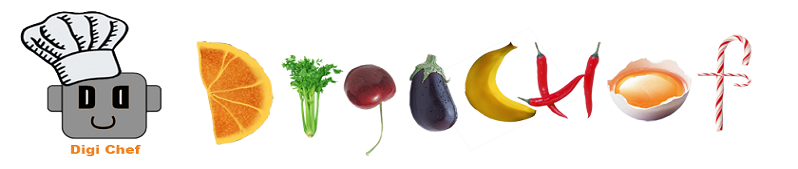
\includegraphics[width=0.9\textwidth]{logowebsite}
\caption{New Logo for Version 2}
\end{center}
\end{figure}

The logo for version 1, however, has been replaced. The new logo (Figure~\ref{fig:logowebsite}) also uses the letters "Digi Chef" as the main part, but instead of just typing them in a simple font, we use several ingredients to sketch up these letters. Therefore, the logo can explain our website's main function, search by ingredients and you will get  recipe for delicious food. 

\subsection{Version 2}

Version 2 is an upgraded version of the original version containing more functions (described by the Product Specification). With the use of technology such as Java Scripts, the web interface looks more polished. 

\begin{figure}[h]
\begin{center}
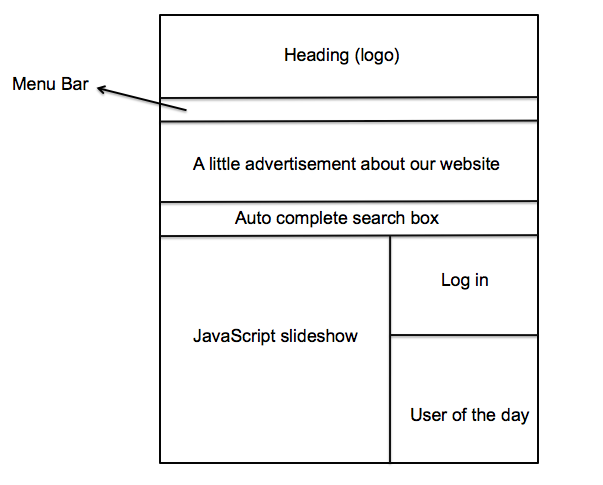
\includegraphics[width=0.9\textwidth]{home_page_v2}
\caption{Layout of the Home Page}
\label{fig:home_page}
\end{center}
\end{figure}

For version 2, our website has a larger database which contains over 900 recipes. For such amount of recipes, it will be a bothering for users if the website still has three drop down boxes for search. Therefore, auto complete search box is used instead. 

\begin{figure}[h]
\begin{center}
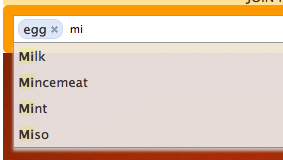
\includegraphics[width=0.6\textwidth]{auto_complete}
\caption{Auto Complete Search Box}
\label{fig:auto_complete}
\end{center}
\end{figure}

As showed in Figure~\ref{fig:auto_complete}, similar to the search result of search server such as Google, once you type in the beginning letter of a word, in this case, an ingredient, the search box will automatically suggest you some related ingredients. Moreover, this search box allow people to search for multiple ingredients (more than three ingredients). In addition, in case of the user does not want an ingredient afterwards, he could simply click "x" to delete it.

Furthermore, for version two, users are allowed to create their own account to rate the recipes. So a register section is presented in the right column of the website, below this section is a part that exhibits the user of the week. 

\begin{figure}[H]
\begin{center}
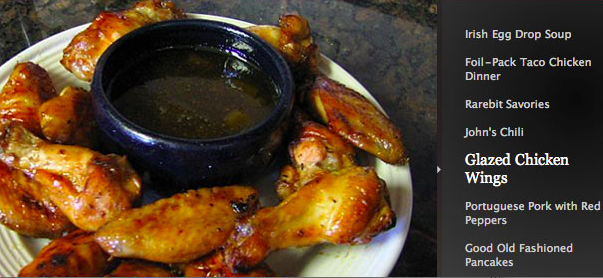
\includegraphics[width=0.9\textwidth]{slideshow}
\caption{Auto Complete Search Box}
\label{fig:slideshow}
\end{center}
\end{figure}

Figure~\ref{fig:slideshow} shows the JavaScript slideshow, the slideshow demonstrates a list of recipes from the database accompany with their image, and each image links to the recipe's own page. As long as the browser is refreshed, the list in the slideshow would change to a new one as well. 

\begin{figure}[H]
\begin{center}
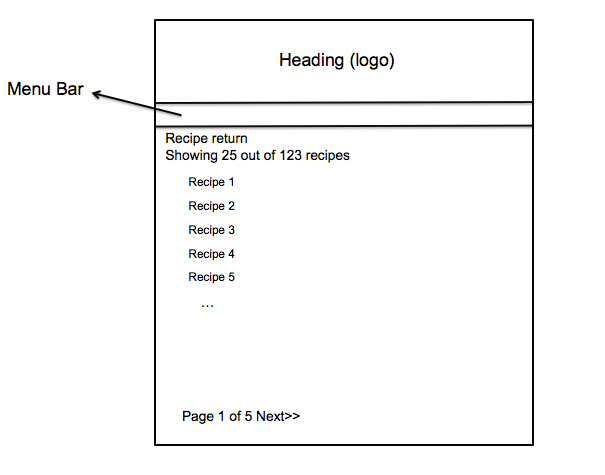
\includegraphics[width=0.9\textwidth]{result_list_v2}
\caption{Layout of the Recipe List Page}
\label{fig:recipe_list_v2}
\end{center}
\end{figure}

Base on the functionality of version 1 and the same serious design of the current interface, the recipe list page (Figure~\ref{fig:recipe_list_v2}) contains a list of recipes with at least one of the searched ingredients. However, the recipe may contain other ingredients which were not specified by the user. Upon recipe selection, the specific recipe page will be displayed.

\begin{figure}[H]
\begin{center}
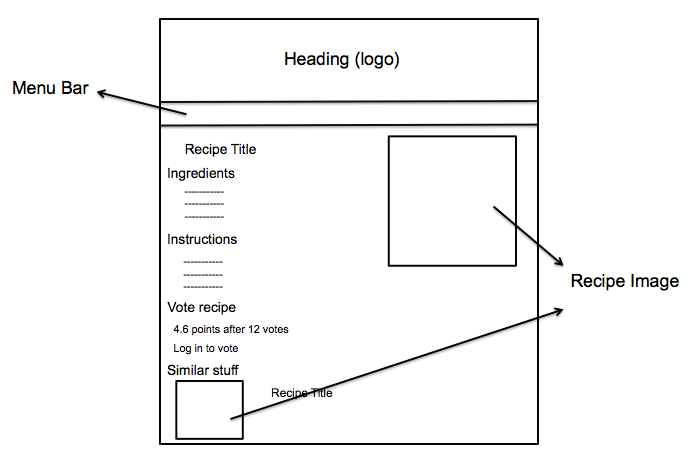
\includegraphics[width=0.9\textwidth]{recipe_page_v2}
\caption{Layout of the Recipe Page}
\label{fig:recipe_page}
\end{center}
\end{figure}

The recipe page (Figure~ \ref{fig:recipe_page_v2}) contains recipe details, for example recipe name, image, ingredients, the instruction, and recipe tags.
 
 With the implement of collaborative filtering, a new section called "Similar Stuff"is added. This section recommend up to five related recipes together with their images. There is also a vote section allow users to rate recipe once they have logged in.
 
 \begin{figure}[H]
 \begin{center}
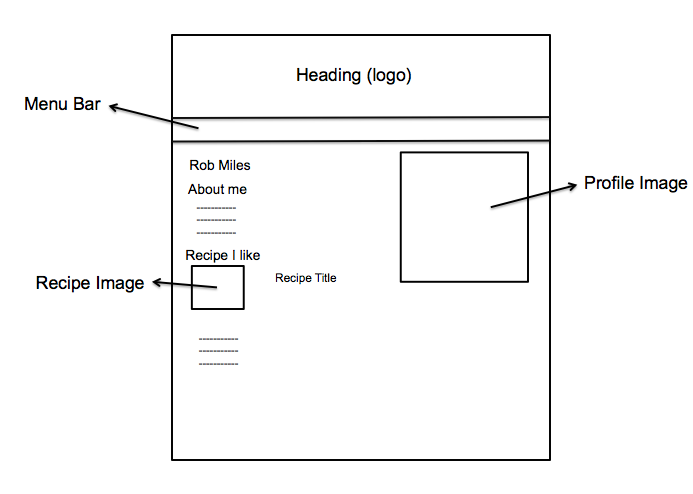
\includegraphics[width=0.9\textwidth]{profile_page_v2}
\caption{Layout of the Profile Page}
\label{fig:profile_page_v2}
\end{center}
\end{figure}

Accessing version 2 of Digi Chef, what user would receive is not only their user account but also their own profile page (Figure~\ref{fig:profile_page_v2}). On the profile page, they can have a section "About me", which describes themselves with a simple sentence even a few words. And a section with some recipes that the user likes at present.

\subsection{Version 3}
The ideal version of our product involves the implementation of a variety of possible functionalities. For instance, for the web based interface, users could choose to click tags and get a list of recipes that contains that particular tag. Additionally, recipes could be made searchable by not just ingredients but also, for example, the type of cuisine (Chinese dish) or whether recipes are vegetarian or non-vegetarian. Moreover, a mobile application could be developed. 

Social networking would be another possibility, with users being able to interact with other users and leave comments on the profile page as well as the recipe page. Users might be able to upload their own recipes and receive ratings from other users. The possibility for improvements are abundant.

